\documentclass[12pt]{article}
\usepackage[margin=3cm]{geometry}

\usepackage{graphicx}
\usepackage{array}
\usepackage{url}
\usepackage{multicol}
\usepackage{amsmath}

\begin{document}

\begin{figure}
    \centering
    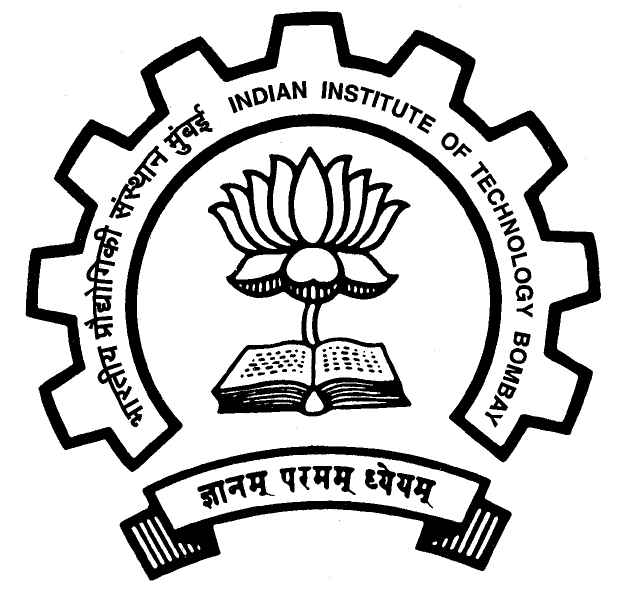
\includegraphics[width=5cm]{iitb-logo.png}
\end{figure}

\begin{center}
    \textbf{\LARGE Indian Institute of Technology Bombay} \\
    \vspace{1cm}
    \Large Project Report\\
    \vspace{0.3cm}

    \rule{\linewidth}{0.5pt} \\
    \vspace{0.2cm}
    \textbf{\LARGE AE 308 \\ \vspace{0.3cm} Control Theory} \\
    \vspace{0.1cm}
    \rule{\linewidth}{0.5pt} \\
    \vspace{1.5cm}
    \LARGE Compensator Design\\

    \vspace{2cm}

    \normalsize Ravi Kumar \\
    210010052

    \vspace{3cm}

    \normalsize\textit{Course Instructor:}\vspace{0.2cm}
    Prof. Arnab Maity

    \vspace{1cm}
    \date{}
\end{center}

\newpage

\section{Introduction}
The given system is a third order type one system with a zero at origin and two
poles at $-10$ and $-1$. The transfer function of the system is given by:
$$G(s) = \dfrac{K}{s(0.1s+1)(s+1)}$$

Bode plot of the system (taking $K=4$):
\begin{figure}[h!]
    \centering
    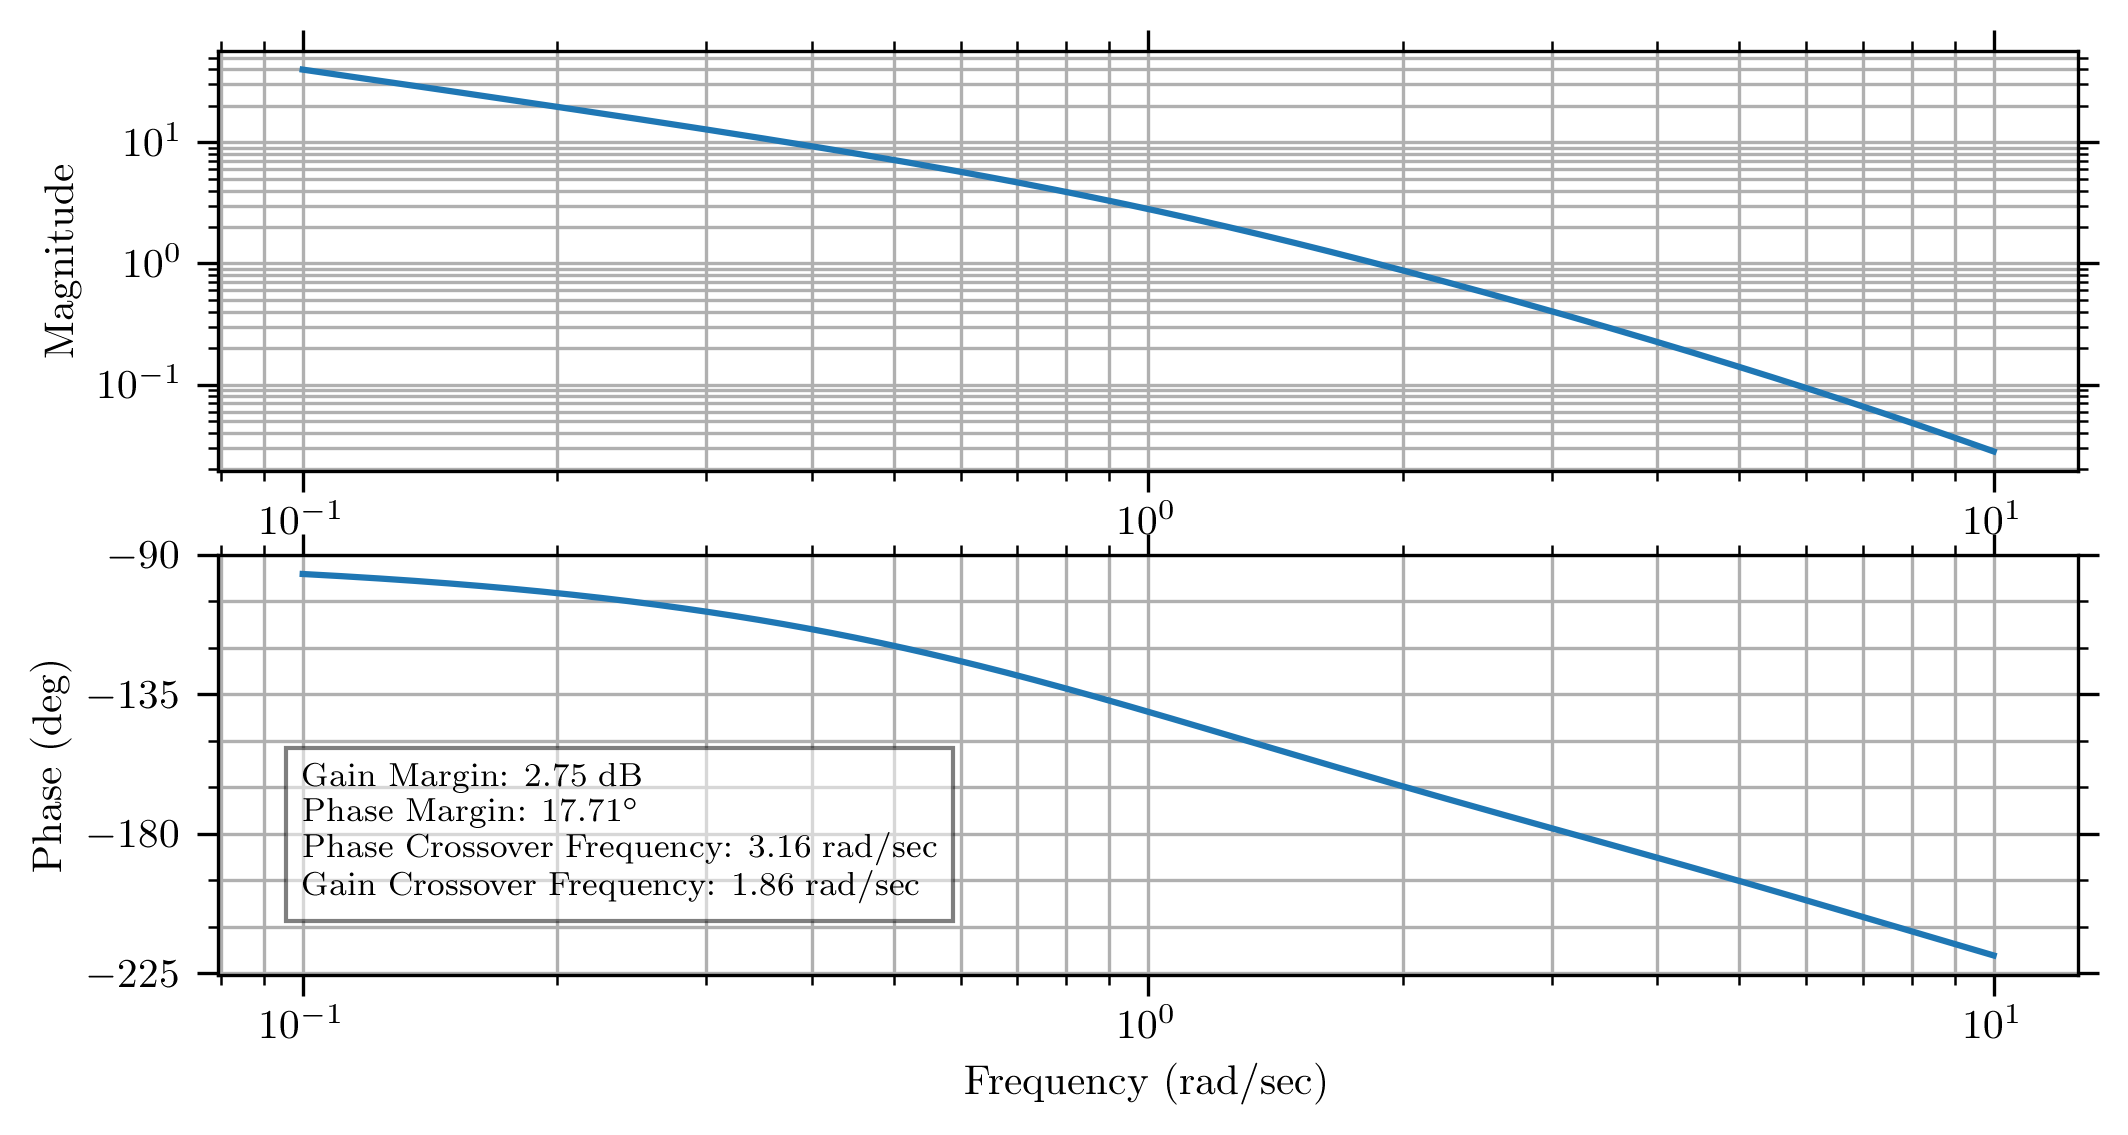
\includegraphics[width=0.8\linewidth]{bode_uncompensated.png}
    \caption {Bode plot of the uncompensated system}
    \label{fig:bode_uncompensated}
\end{figure}

Root locus of the system (taking $K=4$):
\begin{figure}[h!]
    \centering
    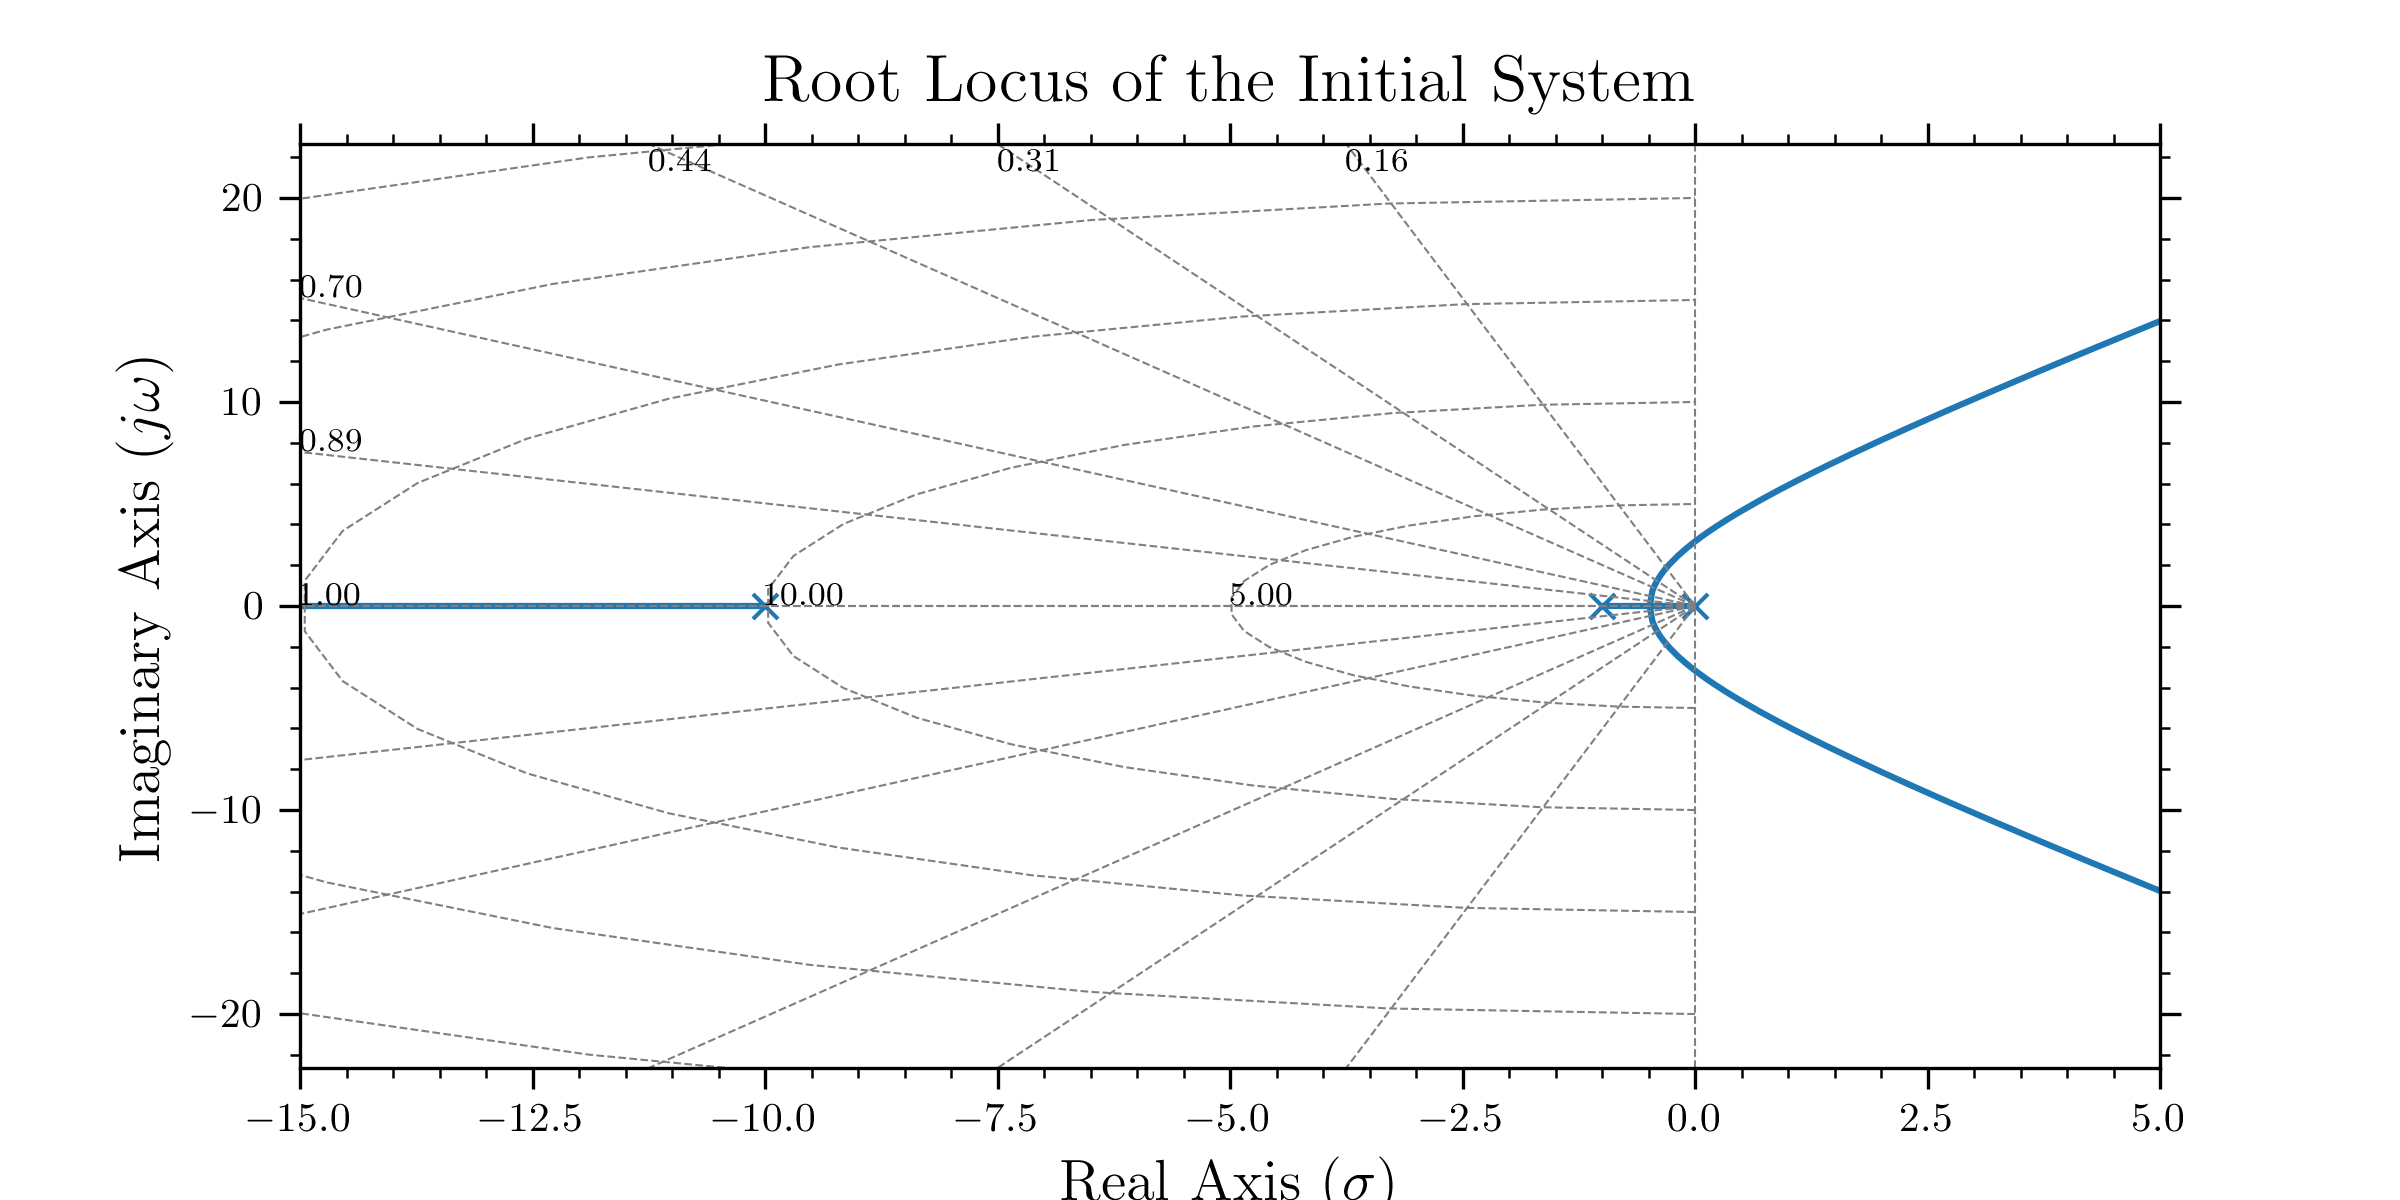
\includegraphics[width=0.8\linewidth]{rootlocus_uncompensated.png}
    \caption {Root locus of the uncompensated system}
    \label{fig:root_locus_uncompensated}
\end{figure}

\clearpage

Step response of the system (taking $K=4$):
\begin{figure}[h!]
    \centering
    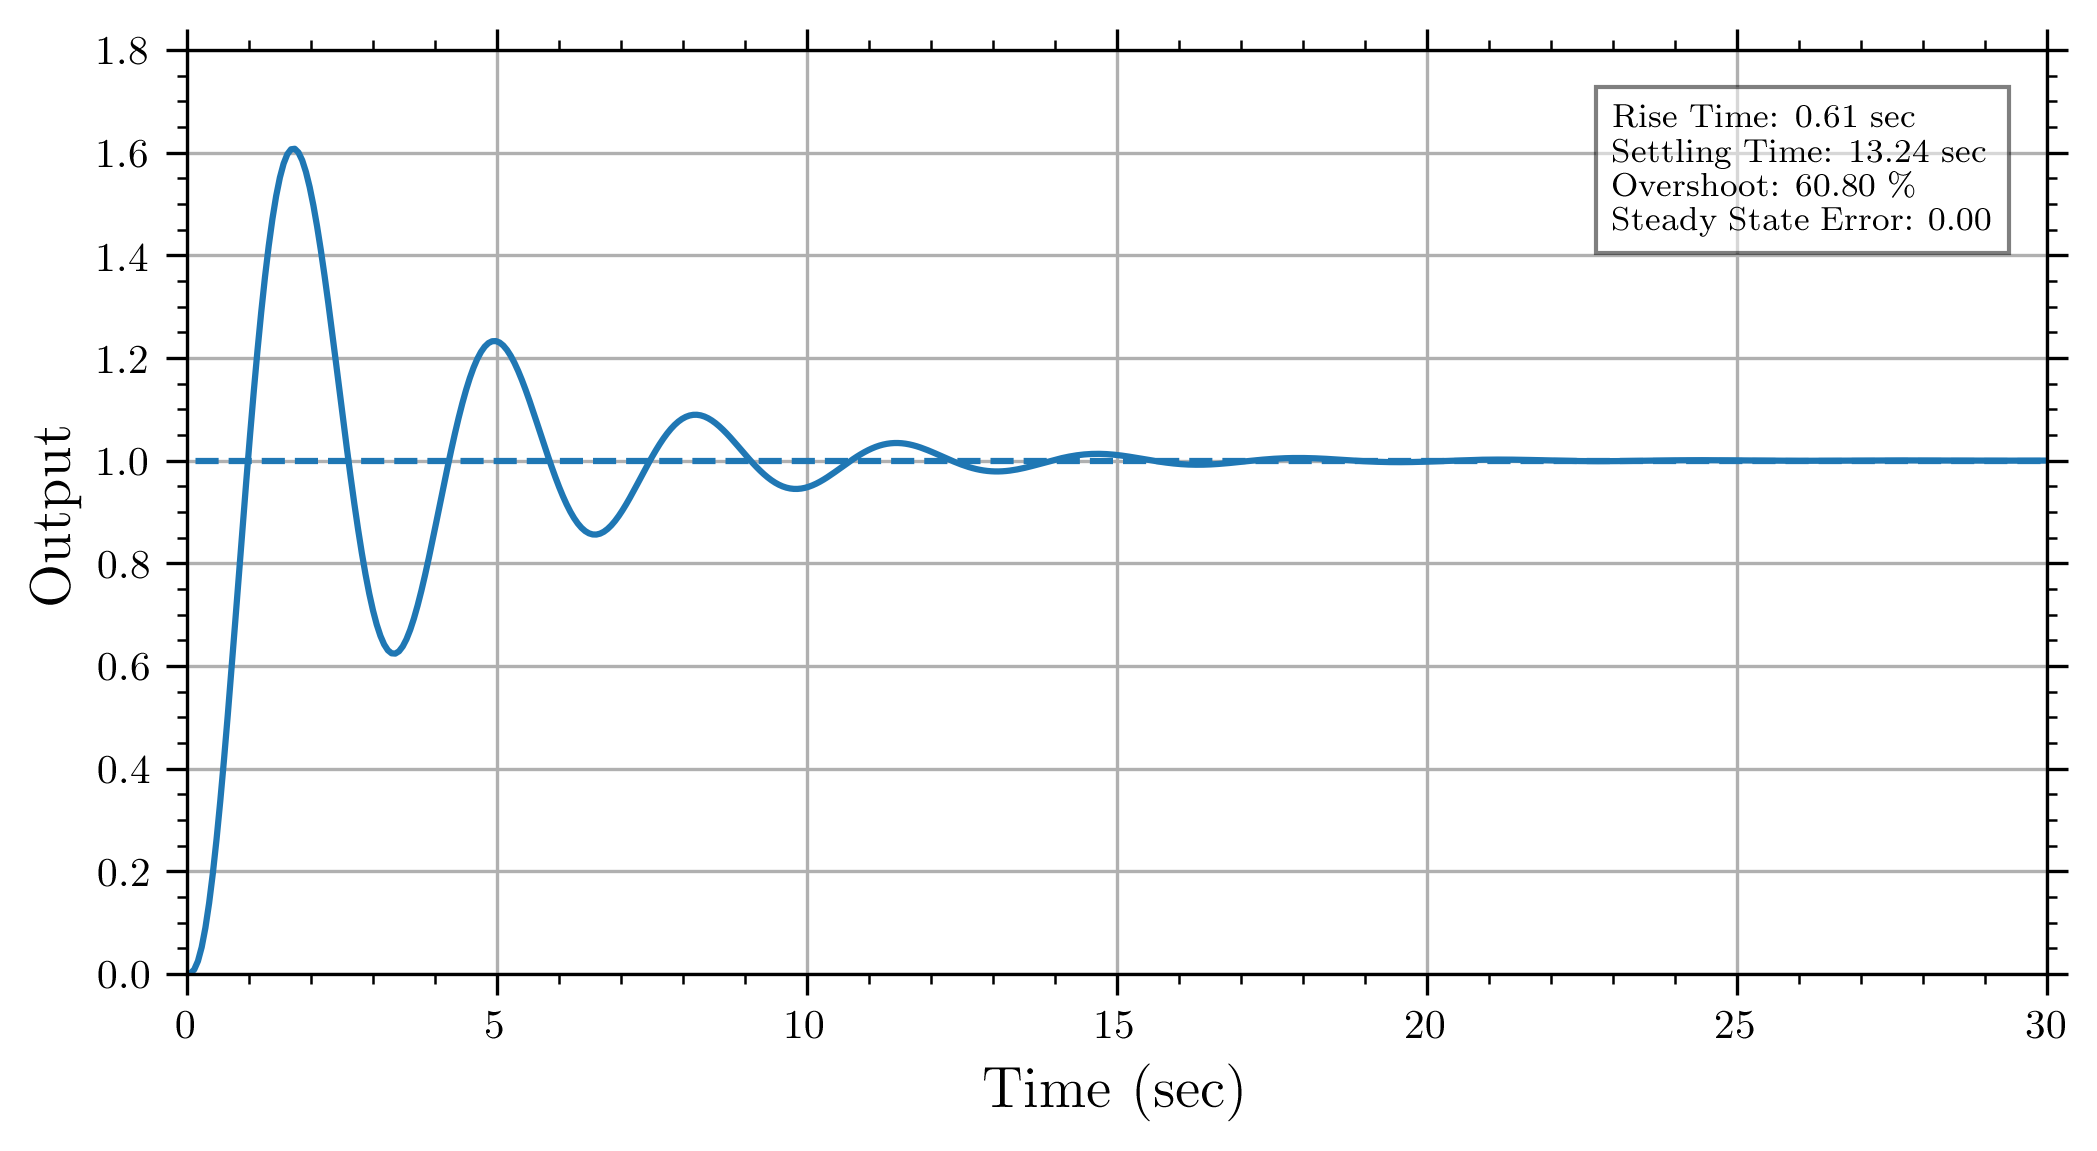
\includegraphics[width=0.8\linewidth]{step_response_uncompensated.png}
    \caption {Step response of the uncompensated system}
    \label{fig:step_uncompensated}
\end{figure}

Ramp response of the system (taking $K=4$):
\begin{figure}[h!]
    \centering
    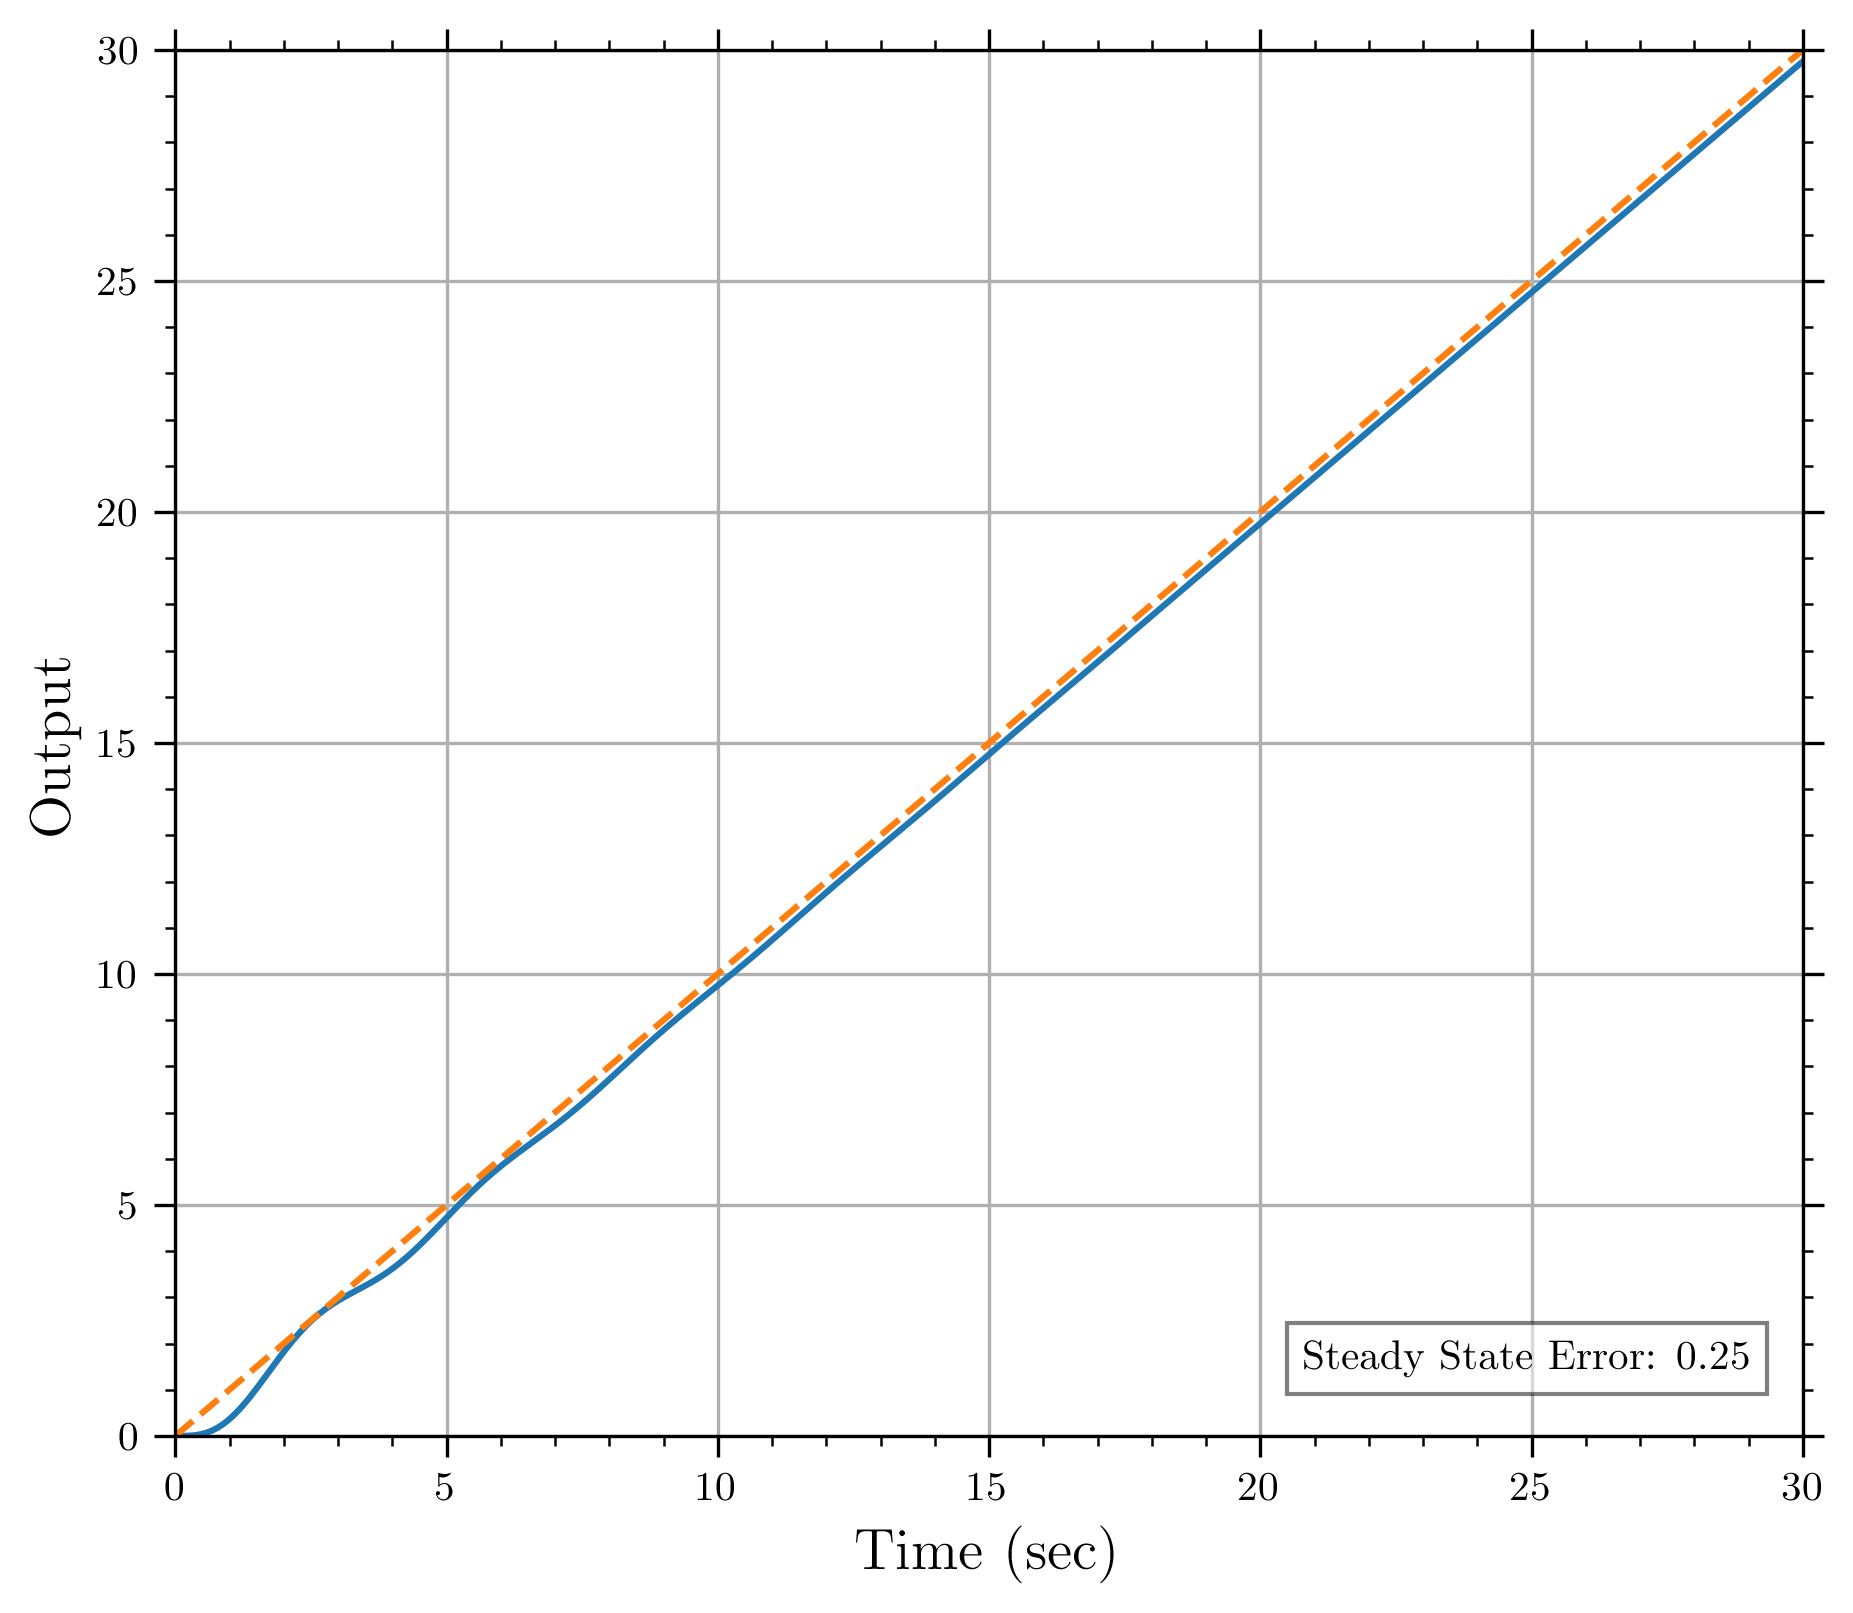
\includegraphics[width=0.7\linewidth]{ramp_response_uncompensated.png}
    \caption {Ramp response of the uncompensated system}
    \label{fig:ramp_uncompensated}
\end{figure}

\clearpage
\section{Control Objectives}
\section{Compensator Design}
\section{Simulation Results}
\section{Conclusion}

\end{document}